%% ============================================================
%% MALTG-WF — Artículo científico formato MDPI (revista Computers)
%% Compilar: pdflatex paper && bibtex paper && pdflatex paper && pdflatex paper
%% ============================================================
\documentclass[computers,article,submit,pdftex,moreauthors]{Definitions/mdpi}

%% Paquetes para figuras y matemáticas
\usepackage{tikz}
\usetikzlibrary{arrows.meta,positioning,shapes.geometric,fit,backgrounds,calc}
\usepackage{pgfplots}
\pgfplotsset{compat=1.17}

%% Castellanización de etiquetas de flotantes
\renewcommand{\figurename}{Figura}
\renewcommand{\tablename}{Tabla}

%% Metadatos del número (placeholder de envío)
\firstpage{1}
\makeatletter
\setcounter{page}{\@firstpage}
\makeatother
\pubvolume{15}
\issuenum{1}
\articlenumber{0}
\pubyear{2026}
\copyrightyear{2026}
\datereceived{ }
\daterevised{ }
\dateaccepted{ }
\datepublished{ }

%% ── Título (mejorado) ──────────────────────────────────────
\Title{MALTG-WF: Arquitectura de Justicia Electrónica Verificable e Interoperable --- Anclaje Ontológico del COGEP para Mitigar Alucinaciones de la IA, Notarización del Expediente por Cadena de Hashes y Apertura Semántica de Datos Judiciales (Caso Ecuador)}

%% ── Autoría (reemplazar con datos definitivos) ─────────────
\newcommand{\orcidauthorA}{0000-0000-0000-0000}
\Author{Patricio Michael~Autor $^{1,}$*}
\AuthorNames{Patricio Michael Autor}
\address{$^{1}$ \quad Programa de Doctorado / Facultad de Ingeniería; correo institucional}
\corres{Correspondencia: pat\_mic@hotmail.com}

%% ── Resumen ────────────────────────────────────────────────
\abstract{Los modelos de lenguaje de gran escala (LLM) alucinan con frecuencia alarmante en el dominio jurídico ---entre el 58\% y el 82\% en consultas de jurisprudencia y aún entre el 17\% y el 33\% en herramientas comerciales con recuperación aumentada---, lo que resulta inadmisible en la tramitación procesal, donde cada afirmación debe ser jurídicamente atribuible. Este artículo propone MALTG-WF, una arquitectura de justicia electrónica que subordina la generación de lenguaje a un razonador simbólico determinista fundado en una ontología ejecutable del Código Orgánico General de Procesos (COGEP) del Ecuador. El flujo procesal se modela como gemelo de flujo BPMN; cada dictamen se deriva exclusivamente del cierre lógico de la base de conocimiento normativa (reglas con artículo, término legal y calendario judicial), de modo que la tasa de alucinación del contenido jurídico emitido es nula por construcción, con procedencia verificable (artículo citado y hash de la base normativa). La integridad de la tramitación entre las partes procesales se asegura con una cadena de hashes SHA-256 que notariza cada actuación (propiedad de evidencia de manipulación demostrada por inducción), y la interoperabilidad con otros sectores de justicia se materializa publicando el expediente como datos abiertos JSON-LD/DCAT. La evaluación sobre 47 causas reales ecuatorianas (procedimientos sumario y monitorio) instancia un flujo canónico de 171 actividades y 79 flujos, evalúa 60 términos procesales (36{,}7\% en plazo; salud procesal media 44{,}4/100) y computa índices de variabilidad fáctica y deriva procesal por causa, demostrando que la transparencia jurídica verificable es alcanzable con componentes abiertos y auditables.}

%% ── Palabras clave ─────────────────────────────────────────
\keyword{alucinaciones de IA; modelos de lenguaje; ontologías jurídicas; COGEP; justicia electrónica; blockchain; cadena de hashes; BPMN; datos abiertos; interoperabilidad; transparencia judicial}

\begin{document}

%% ============================================================
\section{Introducción}
\label{sec:intro}

La incorporación de inteligencia artificial generativa al sector justicia enfrenta una paradoja: los modelos de lenguaje de gran escala (LLM) exhiben una fluidez notable para redactar y resumir textos jurídicos, pero fabrican contenido con una frecuencia incompatible con las garantías del debido proceso. La evidencia empírica es contundente: Dahl et al.\ midieron tasas de alucinación jurídica de entre el 58\% y el 82\% al consultar a LLM generalistas sobre jurisprudencia estadounidense \cite{Dahl2024}, y Magesh et al.\ demostraron que incluso las herramientas comerciales de investigación jurídica con recuperación aumentada (RAG) alucinan entre el 17\% y el 33\% de las veces \cite{Magesh2025}. Las revisiones sistemáticas del fenómeno confirman que la alucinación es una propiedad estructural de la generación neuronal de lenguaje ---no un defecto incidental--- y que su mitigación requiere anclaje a fuentes de conocimiento externas y verificables \cite{Ji2023,Huang2025}. En dominios de alto riesgo, Rudin argumenta que la respuesta correcta no es explicar modelos opacos a posteriori, sino emplear modelos interpretables por diseño \cite{Rudin2019}, posición reforzada por la agenda de la IA explicable responsable \cite{BarredoArrieta2020} y por la convergencia neuro-simbólica que combina redes neuronales con razonamiento lógico \cite{Sarker2021,Pan2024}.

El problema es especialmente crítico en la tramitación procesal, donde tres exigencias convergen: (i) \emph{fidelidad normativa} ---toda afirmación sobre plazos, actos o términos debe derivar de la ley aplicable---; (ii) \emph{integridad del expediente} ---las partes procesales deben poder verificar que ninguna actuación ha sido alterada u omitida---; y (iii) \emph{interoperabilidad} ---otros sectores de justicia (defensoría, fiscalía, academia, veeduría ciudadana) deben poder reutilizar la información sin mediación propietaria. La literatura de e-justicia documenta que los sistemas judiciales electrónicos fallan precisamente en estos frentes por fragmentación técnica y opacidad \cite{Rosa2013,Lupo2014}, mientras que la de gobierno abierto muestra la brecha persistente entre publicar datos y hacerlos reutilizables \cite{Janssen2012,Attard2015}.

Este artículo aborda las tres exigencias con una arquitectura integrada, MALTG-WF, construida sobre el módulo de flujo procesal (WORKFLOW) de la plataforma MALTG y validada con datos reales del sistema procesal civil ecuatoriano regido por el Código Orgánico General de Procesos (COGEP). La tesis central es que, en el dominio procesal, la alucinación no debe \emph{corregirse} sino \emph{excluirse por construcción}: el contenido jurídico de toda respuesta se genera mediante un razonador simbólico determinista sobre una ontología ejecutable del COGEP ---con reglas que citan artículo, término legal en días hábiles y calendario judicial oficial---, y el LLM queda relegado a tareas de superficie lingüística sin autoridad para introducir hechos ni normas. Cada dictamen porta su procedencia (artículo aplicado, fechas comparadas, hash criptográfico de la base normativa), cada actuación queda notarizada en una cadena de hashes con evidencia de manipulación \cite{Haber1991}, y cada expediente se publica como datos abiertos JSON-LD/DCAT \cite{Bizer2009,Guha2016}.

Las contribuciones son cinco:
\begin{enumerate}
\item Un \textbf{modelo formal} del flujo procesal como gemelo BPMN con base de conocimiento normativa ejecutable $\Omega_{L}$, función de veredicto por términos legales en días hábiles y métricas agregadas de salud procesal, variabilidad fáctica y deriva de proceso (Sección~\ref{sec:formal}).
\item Una \textbf{barrera anti-alucinación} (guardrail) formalizada: el conjunto de respuestas emitibles se restringe al cierre lógico de $\Omega_{L}$ y los hechos del expediente, con proposición de fidelidad por construcción y procedencia auditable (Sección~\ref{sec:formal}).
\item Un \textbf{esquema de notarización} del expediente mediante cadena de hashes SHA-256 con demostración por inducción de la propiedad de evidencia de manipulación, en la tradición del sellado temporal criptográfico \cite{Haber1991} y de los libros mayores distribuidos \cite{Zheng2018,Casino2019} (Sección~\ref{sec:formal}).
\item Una \textbf{arquitectura de referencia} contenedorizada que integra el gemelo de flujo, el razonador, la barrera, el libro mayor y la publicación de datos abiertos (Sección~\ref{sec:arch}).
\item Una \textbf{evaluación empírica} con 47 causas reales ecuatorianas: 60 términos procesales evaluados, salud media 44{,}4/100, índice global de puntualidad 36{,}7\%, y diagnóstico por procedimiento (Sección~\ref{sec:results}).
\end{enumerate}

%% ============================================================
\section{Trabajo Relacionado}
\label{sec:related}

\subsection{Alucinaciones de los LLM y Anclaje de Conocimiento}
La taxonomía de Ji et al.\ distingue alucinación intrínseca (contradicción con la fuente) y extrínseca (contenido no verificable) \cite{Ji2023}; Huang et al.\ la extienden a los LLM contemporáneos, distinguiendo alucinación de facticidad y de fidelidad \cite{Huang2025}. En el ámbito jurídico, Dahl et al.\ aportan la primera cuantificación sistemática \cite{Dahl2024} y Magesh et al.\ evidencian que la recuperación aumentada reduce pero no elimina el fenómeno \cite{Magesh2025}. La integración de LLM con grafos de conocimiento se perfila como la vía principal de mitigación \cite{Pan2024,Hogan2021}, dentro del programa neuro-simbólico general \cite{Sarker2021}. Nuestra posición es más restrictiva que la RAG: en lugar de \emph{informar} al generador con documentos recuperados, el contenido jurídico se \emph{deriva} simbólicamente y el generador no puede alterarlo, en sintonía con el principio de interpretabilidad por diseño para decisiones de alto riesgo \cite{Rudin2019,BarredoArrieta2020}.

\subsection{Ontologías Jurídicas y Flujos Procesales}
La comunidad de IA y derecho acumula tres décadas de ontologías y razonadores normativos \cite{BenchCapon2012,Casanovas2016}, con fundamentos clásicos de ingeniería ontológica \cite{Gruber1993,Uschold1996}. El aprendizaje automático predictivo sobre decisiones judiciales \cite{Katz2017,Medvedeva2020} opera, sin embargo, como caja negra, y no ofrece las garantías de atribución que exige la tramitación. En paralelo, la gestión de procesos de negocio proporciona el aparato para modelar flujos procesales: BPMN como estándar de modelado \cite{Chinosi2012}, el ciclo de vida BPM \cite{Aalst2013} y la verificación de conformidad entre el modelo canónico y las trazas reales \cite{Rozinat2008}, que nuestro índice de variabilidad fáctica adapta al expediente judicial.

\subsection{Blockchain y Datos Abiertos en el Sector Justicia}
El sellado temporal criptográfico de documentos precede al blockchain moderno \cite{Haber1991}; las revisiones de Zheng et al.\ y Casino et al.\ sistematizan sus variantes y aplicaciones \cite{Zheng2018,Casino2019}, Ølnes et al.\ analizan su valor específico para el sector público ---integridad y no repudio de registros compartidos--- \cite{Olnes2017}, y Christidis y Devetsikiotis formalizan los contratos inteligentes \cite{Christidis2016}, cuya relación con los contratos legales ha sido estudiada en profundidad por Governatori et al.\ \cite{Governatori2018}. En cuanto a la apertura, los principios de datos enlazados \cite{Bizer2009}, la experiencia de Schema.org \cite{Guha2016} y los principios FAIR \cite{Wilkinson2016} definen el estándar de interoperabilidad que la e-justicia aún no alcanza \cite{Rosa2013,Lupo2014}. La Tabla~\ref{tab:related} posiciona nuestra contribución.

\begin{table}[H]
\caption{Comparación con líneas de trabajo próximas respecto a las garantías ofrecidas.}
\label{tab:related}
\begin{tabularx}{\textwidth}{lXXXX}
\toprule
\textbf{Enfoque} & \textbf{Fidelidad normativa} & \textbf{Integridad del expediente} & \textbf{Interoperabilidad semántica} & \textbf{Explicabilidad}\\
\midrule
LLM generalista \cite{Dahl2024} & No (58--82\% aluc.) & No & No & No\\
RAG jurídico comercial \cite{Magesh2025} & Parcial (17--33\% aluc.) & No & No & Parcial\\
ML predictivo \cite{Katz2017,Medvedeva2020} & No aplica & No & No & No\\
LLM + grafos de conocimiento \cite{Pan2024} & Parcial & No & Sí & Parcial\\
Blockchain gubernamental \cite{Olnes2017} & No aplica & Sí & Parcial & No aplica\\
\textbf{MALTG-WF (este trabajo)} & \textbf{Sí (0\% por construcción)} & \textbf{Sí (cadena de hashes)} & \textbf{Sí (JSON-LD/DCAT)} & \textbf{Sí (regla y artículo)}\\
\bottomrule
\end{tabularx}
\end{table}

%% ============================================================
\section{Modelo Formal}
\label{sec:formal}

\subsection{Gemelo de Flujo Procesal y Base de Conocimiento Normativa}

\begin{Definition}[Gemelo de flujo BPMN]
El flujo canónico de un procedimiento es un grafo dirigido $W = (A, F, S, \lambda)$, donde $A$ es el conjunto de actividades y eventos procesales, $F \subseteq A \times A$ los flujos de secuencia, $S$ la partición de $A$ en etapas procesales (calles BPMN \cite{Chinosi2012}) y $\lambda$ el etiquetado con metadatos (término legal, nota, artículo). Una causa $c$ induce una traza $\tau(c) = \langle (a_1, t_1), \dots, (a_m, t_m) \rangle$ de actuaciones fechadas, ordenada cronológicamente.
\end{Definition}

\begin{Definition}[Ontología ejecutable del COGEP]
La base de conocimiento normativa es la tupla $\Omega_{L} = \langle \Pi, \mathcal{A}, \mathcal{R}, H \rangle$: $\Pi$ es el catálogo de procedimientos (sumario, ordinario, monitorio, ejecutivo, apelación, ejecución, voluntario); $\mathcal{A}$ el catálogo de actos procesales tipificados con patrones de reconocimiento; $\mathcal{R}$ el conjunto de reglas de término, donde cada regla es una tupla
\begin{equation}
r = \langle a_{\mathrm{desde}},\, a_{\mathrm{hasta}},\, T_r,\, \mathrm{art}_r,\, \Pi_r \rangle,
\label{eq:regla}
\end{equation}
con actos de origen y destino, término legal $T_r$ en días hábiles, artículo COGEP que la fundamenta y procedimientos $\Pi_r \subseteq \Pi$ donde aplica; y $H$ el calendario judicial (fines de semana y feriados oficiales).
\end{Definition}

El tiempo procesal se computa en días hábiles conforme al calendario:
\begin{equation}
d_H(t_1, t_2) \;=\; \bigl|\{\, t \in (t_1, t_2] : t \notin H \,\}\bigr|.
\label{eq:habiles}
\end{equation}

\begin{Definition}[Veredicto de término]
Sea $r \in \mathcal{R}$ aplicable a la causa $c$, con primeras ocurrencias fechadas de sus actos $t_{\mathrm{desde}} < t_{\mathrm{hasta}}$, y sea $d = d_H(t_{\mathrm{desde}}, t_{\mathrm{hasta}})$. Con factor de tolerancia $\alpha = 1{,}25$, el veredicto es la función escalonada
\begin{equation}
V(r, c) \;=\;
\begin{cases}
\textsc{cumple}, & d \le T_r,\\[2pt]
\textsc{alerta}, & T_r < d \le \alpha\, T_r,\\[2pt]
\textsc{incumple}, & d > \alpha\, T_r,
\end{cases}
\qquad
\pi(V) = \begin{cases} 100\\ 60\\ 0 \end{cases}
\label{eq:verdict}
\end{equation}
y la \emph{salud procesal} de la causa es la media de puntos sobre las reglas evaluables $\mathcal{R}_c$:
\begin{equation}
S(c) \;=\; \frac{1}{|\mathcal{R}_c|} \sum_{r \in \mathcal{R}_c} \pi\bigl(V(r,c)\bigr) \;\in\; [0, 100].
\label{eq:salud}
\end{equation}
\end{Definition}

Dos métricas complementarias cuantifican la desviación estructural de la traza respecto al flujo canónico, adaptando la verificación de conformidad de procesos \cite{Rozinat2008}. El \emph{índice de variabilidad fáctica} compara los actos observados con los canónicos del procedimiento,
\begin{equation}
\mathrm{IVF}(c) \;=\; 100 \cdot \frac{|E_c| + |M_c|}{|K_c| + |E_c|},
\label{eq:ivf}
\end{equation}
con $K_c$ los actos canónicos observados, $E_c$ los actos fuera del flujo canónico y $M_c$ los canónicos faltantes; y el \emph{índice de deriva procesal} $\mathrm{IDP}(c) \in [0,100]$ acumula puntos por patrones anómalos detectados en $\tau(c)$ (bucles, alternancia \emph{ping-pong}, estancamiento legal y retroceso de etapa). El \emph{riesgo} agregado de la causa pondera las tres señales:
\begin{equation}
\rho(c) \;=\; w_s \bigl(100 - S(c)\bigr) + w_v\, \mathrm{IVF}(c) + w_d\, \mathrm{IDP}(c),
\qquad (w_s, w_v, w_d) = (0{,}50,\, 0{,}25,\, 0{,}25).
\label{eq:riesgo}
\end{equation}

\subsection{Barrera Anti-Alucinación por Anclaje Ontológico}

Sea $F_c$ el conjunto de hechos del expediente $c$ (actuaciones, fechas, cabecera) y $\mathrm{Th}(\Omega_L \cup F_c)$ el cierre de consecuencias derivables por el razonador determinista (aplicación de las ecuaciones \eqref{eq:habiles}--\eqref{eq:riesgo}). Toda interacción en lenguaje natural se procesa en dos fases: una función de interpretación $\iota$ asigna la consulta del usuario a una intención tipificada (plazos, salud, integridad, historial, apertura de datos), y el contenido de la respuesta se construye exclusivamente con elementos de $\mathrm{Th}(\Omega_L \cup F_c)$; la generación lingüística solo da forma superficial a ese contenido.

\begin{Definition}[Tasa de alucinación emitida]
Si $\mathcal{C}(y)$ es el conjunto de afirmaciones jurídicas verificables contenidas en una respuesta $y$, la tasa de alucinación de un sistema sobre un conjunto de consultas $Q$ es
\begin{equation}
\mathcal{H} \;=\; \frac{\bigl|\{\, q \in Q : \exists\, \phi \in \mathcal{C}(y_q),\; \phi \notin \mathrm{Th}(\Omega_L \cup F_c) \,\}\bigr|}{|Q|}.
\label{eq:hall}
\end{equation}
\end{Definition}

\begin{Proposition}[Fidelidad por construcción]
En MALTG-WF, $\mathcal{H} = 0$ sobre el dominio de intenciones tipificadas. Además, toda afirmación emitida $\phi$ porta procedencia verificable: la regla $r$ y el artículo $\mathrm{art}_r$ que la fundamentan, las fechas comparadas y el resumen criptográfico $h(\Omega_L)$ de la base normativa vigente al momento del dictamen.
\end{Proposition}

\begin{proof}
Por construcción, el canal de generación no dispone de mecanismo para introducir afirmaciones fuera de $\mathrm{Th}(\Omega_L \cup F_c)$: las plantillas de respuesta se instancian únicamente con salidas del razonador, que es determinista y total sobre las intenciones tipificadas. Para la procedencia, cada elemento de $\mathrm{Th}$ conserva el identificador de la regla y las fechas de las que deriva (ecuaciones \eqref{eq:regla}--\eqref{eq:verdict}), y $h(\Omega_L)$ se publica con cada dictamen, lo que permite a un tercero re-derivar $\phi$ y detectar cualquier cambio normativo. Las consultas fuera del dominio tipificado se rechazan explícitamente en lugar de responderse, preservando $\mathcal{H}=0$ a costa de cobertura.
\end{proof}

Esta garantía invierte el compromiso de los sistemas RAG: donde aquellos maximizan cobertura tolerando alucinación residual \cite{Magesh2025}, MALTG-WF maximiza fidelidad acotando la cobertura al dominio normativo formalizado, el criterio apropiado cuando la respuesta incide en derechos procesales \cite{Rudin2019}.

\subsection{Notarización del Expediente por Cadena de Hashes}

\begin{Definition}[Cadena de custodia criptográfica]
Sea $\tau(c) = \langle x_0, \dots, x_{m-1} \rangle$ la secuencia cronológica de actuaciones y $h$ una función resumen criptográfica (SHA-256). Con $b_{-1} = 0^{256}$, el bloque $i$-ésimo es
\begin{equation}
b_i \;=\; h\bigl(\, i \,\|\, t_i \,\|\, h(x_i) \,\|\, b_{i-1} \,\bigr), \qquad i = 0, \dots, m-1,
\label{eq:chain}
\end{equation}
y la raíz del expediente es $b_{m-1}$. La publicación de $b_{m-1}$ ante las partes procesales notariza el estado íntegro del expediente \cite{Haber1991}.
\end{Definition}

\begin{Proposition}[Evidencia de manipulación]
Si un adversario sustituye la actuación $x_j$ por $x'_j \neq x_j$ (o altera su fecha $t_j$ o su posición $j$), entonces $b'_k \neq b_k$ para todo $k \geq j$ salvo con probabilidad despreciable ($\le 2^{-128}$ por resistencia a colisiones de SHA-256); en particular, la raíz cambia y la alteración es detectable por cualquier parte que conserve $b_{m-1}$.
\end{Proposition}

\begin{proof}
Por inducción sobre $k$. \emph{Base}: para $k = j$, si $x'_j \neq x_j$ entonces $h(x'_j) \neq h(x_j)$ salvo colisión, y $b'_j = h(j \| t_j \| h(x'_j) \| b_{j-1}) \neq b_j$ salvo colisión de la composición. \emph{Paso}: si $b'_{k-1} \neq b_{k-1}$, el argumento de $h$ en \eqref{eq:chain} difiere en el cuarto componente, luego $b'_k \neq b_k$ salvo colisión. La unión de los sucesos de colisión sobre $m$ bloques mantiene probabilidad despreciable para $m$ polinómico.
\end{proof}

El mismo principio de encadenamiento gobierna la bitácora de auditoría del sistema (registro de solo escritura de ingestas, dictámenes y accesos), de modo que la plataforma completa ---no solo el expediente--- es auditable. Este esquema constituye la capa mínima verificable de un despliegue de libro mayor distribuido: la raíz $b_{m-1}$ puede anclarse periódicamente en una red DLT permisionada interinstitucional \cite{Olnes2017,Christidis2016} sin modificar el modelo formal.

\subsection{Apertura Semántica del Expediente}

La interoperabilidad con otros sectores de justicia se formaliza como una proyección $\mathcal{O}: (F_c, \mathrm{Th}) \rightarrow \mathrm{JSON\text{-}LD}$ que publica cabecera y actuaciones con vocabularios estándar (Schema.org, Dublin Core, DCAT) \cite{Guha2016,Bizer2009}, licencia abierta y declaración de conformidad normativa (\texttt{dct:conformsTo} = COGEP), satisfaciendo los principios FAIR de localizabilidad, accesibilidad, interoperabilidad y reutilización \cite{Wilkinson2016}. La Tabla~\ref{tab:opendata} detalla el mapeo.

\begin{table}[H]
\caption{Proyección del expediente judicial a datos abiertos JSON-LD/DCAT.}
\label{tab:opendata}
\begin{tabularx}{\textwidth}{llX}
\toprule
\textbf{Elemento del expediente} & \textbf{Término semántico} & \textbf{Función de interoperabilidad}\\
\midrule
Identificador de la causa & \texttt{schema:identifier} & Clave de enlace intersectorial.\\
Materia y tipo de acción & \texttt{schema:about} / \texttt{dct:title} & Clasificación temática reutilizable.\\
Judicatura & \texttt{schema:provider} & Atribución institucional.\\
Fecha de ingreso & \texttt{dct:created} & Serie temporal procesal.\\
Actuación procesal & \texttt{schema:Action} (+ posición y fecha) & Traza $\tau(c)$ legible por máquina.\\
Conformidad normativa & \texttt{dct:conformsTo} (COGEP) & Contexto jurídico explícito.\\
Licencia & \texttt{dct:license} (CC BY 4.0) & Reutilización por defensoría, academia, veeduría.\\
Conjunto de datos & \texttt{dcat:Dataset} + \texttt{dcat:landingPage} & Catalogación en portales de datos abiertos \cite{Attard2015}.\\
\bottomrule
\end{tabularx}
\end{table}

%% ============================================================
\section{Arquitectura MALTG-WF}
\label{sec:arch}

La Figura~\ref{fig:arch} presenta la arquitectura, desplegada como contenedores Docker con una API REST (FastAPI) y un frontend de visualización que renderiza el gemelo de flujo BPMN con las causas superpuestas. El recorrido de una consulta ilustra la integración: (1) el expediente ---obtenido del sistema público de consulta de procesos--- se serializa como JSON-LD y alimenta el gemelo de flujo; (2) el razonador COGEP aplica las reglas de $\Omega_L$ y produce dictámenes con procedencia; (3) la barrera anti-alucinación restringe toda respuesta en lenguaje natural al contenido derivado (Figura~\ref{fig:guardrail}); (4) el libro mayor encadena las actuaciones (Figura~\ref{fig:chain}) y la bitácora registra la operación; y (5) el expediente y sus dictámenes se publican como datos abiertos. El ciclo de supervisión sigue el patrón MAPE-K de la computación autonómica \cite{Kephart2003}, con la decisión final siempre reservada al operador jurídico humano.

\begin{figure}[H]
\centering
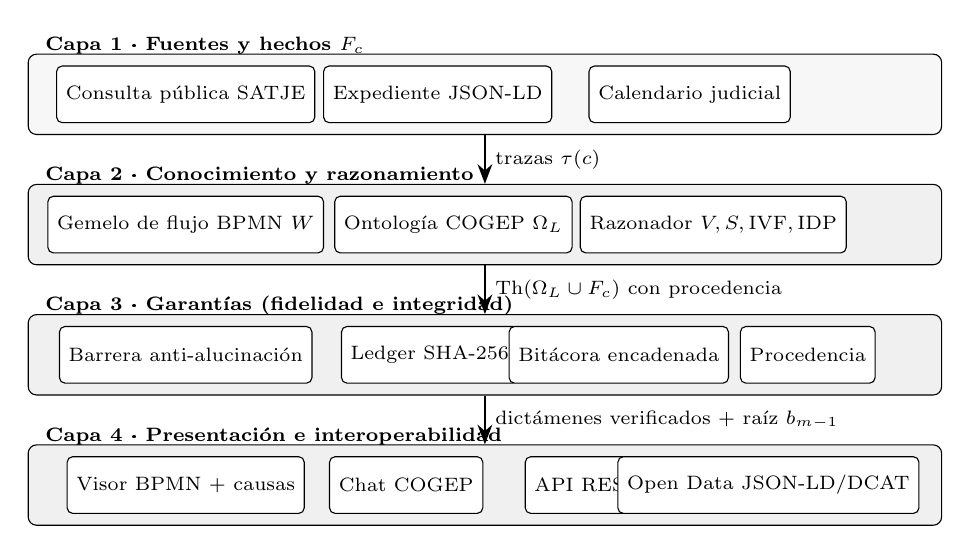
\begin{tikzpicture}[
  capa/.style={draw, rounded corners=3pt, minimum width=11.6cm, minimum height=1.02cm, align=center, font=\small},
  comp/.style={draw, rounded corners=2pt, minimum height=0.72cm, align=center, font=\scriptsize, fill=white},
  flow/.style={-{Stealth[length=2.5mm]}, thick},
  node distance=0.42cm]
\node[capa, fill=gray!6]  (l1) {};
\node[comp] at ($(l1.center)+(-3.8,0)$) {Consulta pública SATJE};
\node[comp] at ($(l1.center)+(-0.6,0)$) {Expediente JSON-LD};
\node[comp] at ($(l1.center)+(2.6,0)$)  {Calendario judicial};
\node[font=\scriptsize\bfseries, anchor=west] at ($(l1.west)+(0.1,0.62)$) {Capa 1 · Fuentes y hechos $F_c$};

\node[capa, below=0.62cm of l1, fill=gray!12] (l2) {};
\node[comp] at ($(l2.center)+(-3.8,0)$) {Gemelo de flujo BPMN $W$};
\node[comp] at ($(l2.center)+(-0.4,0)$) {Ontología COGEP $\Omega_L$};
\node[comp] at ($(l2.center)+(2.9,0)$)  {Razonador $V, S, \mathrm{IVF}, \mathrm{IDP}$};
\node[font=\scriptsize\bfseries, anchor=west] at ($(l2.west)+(0.1,0.62)$) {Capa 2 · Conocimiento y razonamiento};

\node[capa, below=0.62cm of l2, fill=gray!12] (l3) {};
\node[comp] at ($(l3.center)+(-3.8,0)$) {Barrera anti-alucinación};
\node[comp] at ($(l3.center)+(-0.7,0)$) {Ledger SHA-256};
\node[comp] at ($(l3.center)+(1.7,0)$)  {Bitácora encadenada};
\node[comp] at ($(l3.center)+(4.1,0)$)  {Procedencia};
\node[font=\scriptsize\bfseries, anchor=west] at ($(l3.west)+(0.1,0.62)$) {Capa 3 · Garantías (fidelidad e integridad)};

\node[capa, below=0.62cm of l3, fill=gray!12] (l4) {};
\node[comp] at ($(l4.center)+(-3.8,0)$) {Visor BPMN + causas};
\node[comp] at ($(l4.center)+(-1.0,0)$) {Chat COGEP};
\node[comp] at ($(l4.center)+(1.3,0)$)  {API REST};
\node[comp] at ($(l4.center)+(3.6,0)$)  {Open Data JSON-LD/DCAT};
\node[font=\scriptsize\bfseries, anchor=west] at ($(l4.west)+(0.1,0.62)$) {Capa 4 · Presentación e interoperabilidad};

\draw[flow] (l1) -- node[right, font=\scriptsize]{trazas $\tau(c)$} (l2);
\draw[flow] (l2) -- node[right, font=\scriptsize]{$\mathrm{Th}(\Omega_L \cup F_c)$ con procedencia} (l3);
\draw[flow] (l3) -- node[right, font=\scriptsize]{dictámenes verificados + raíz $b_{m-1}$} (l4);
\end{tikzpicture}
\caption{Arquitectura MALTG-WF. El contenido jurídico fluye siempre a través del razonador y de la capa de garantías; ningún componente generativo accede directamente a la capa de presentación.}
\label{fig:arch}
\end{figure}

\begin{figure}[H]
\centering
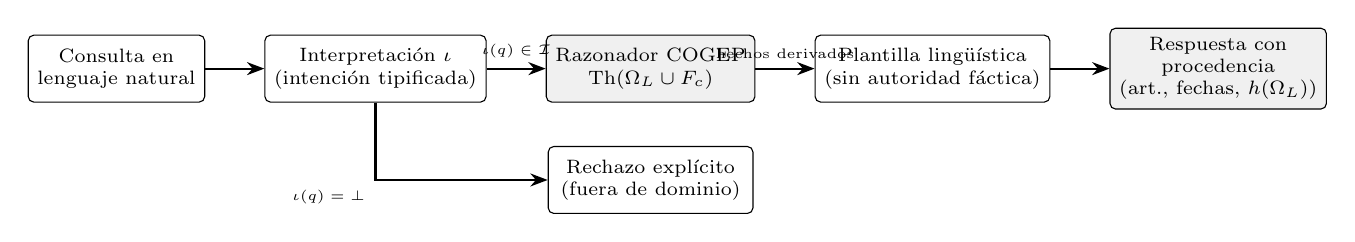
\begin{tikzpicture}[
  box/.style={draw, rounded corners=2pt, align=center, font=\scriptsize, minimum height=0.85cm},
  flow/.style={-{Stealth[length=2.2mm]}, thick},
  node distance=0.55cm and 0.75cm]
\node[box, minimum width=2.2cm] (q) {Consulta en\\lenguaje natural};
\node[box, right=of q, minimum width=2.2cm] (i) {Interpretación $\iota$\\(intención tipificada)};
\node[box, right=of i, minimum width=2.6cm, fill=gray!12] (r) {Razonador COGEP\\$\mathrm{Th}(\Omega_L \cup F_c)$};
\node[box, right=of r, minimum width=2.4cm] (t) {Plantilla lingüística\\(sin autoridad fáctica)};
\node[box, below=of r, minimum width=2.6cm] (rej) {Rechazo explícito\\(fuera de dominio)};
\node[box, right=of t, minimum width=2.0cm, fill=gray!12] (y) {Respuesta con\\procedencia\\(art., fechas, $h(\Omega_L)$)};
\draw[flow] (q) -- (i);
\draw[flow] (i) -- node[above, font=\tiny]{$\iota(q) \in \mathcal{I}$} (r);
\draw[flow] (i) |- node[below left, font=\tiny]{$\iota(q) = \bot$} (rej);
\draw[flow] (r) -- node[above, font=\tiny]{hechos derivados} (t);
\draw[flow] (t) -- (y);
\end{tikzpicture}
\caption{Barrera anti-alucinación. El contenido jurídico procede únicamente del cierre lógico $\mathrm{Th}(\Omega_L \cup F_c)$; las consultas no tipificadas se rechazan en lugar de responderse, garantizando $\mathcal{H}=0$ (ecuación \eqref{eq:hall}).}
\label{fig:guardrail}
\end{figure}

\begin{figure}[H]
\centering
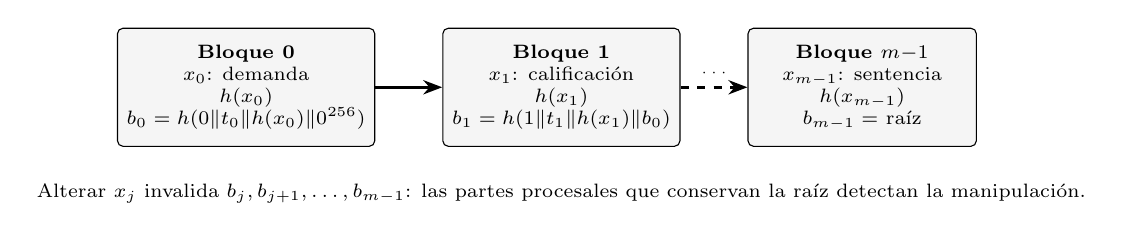
\begin{tikzpicture}[
  blk/.style={draw, rounded corners=2pt, align=center, font=\scriptsize, minimum width=2.9cm, minimum height=1.5cm, fill=gray!8},
  flow/.style={-{Stealth[length=2.4mm]}, very thick},
  node distance=0.85cm]
\node[blk] (b0) {\textbf{Bloque 0}\\$x_0$: demanda\\$h(x_0)$\\$b_0 = h(0 \| t_0 \| h(x_0) \| 0^{256})$};
\node[blk, right=of b0] (b1) {\textbf{Bloque 1}\\$x_1$: calificación\\$h(x_1)$\\$b_1 = h(1 \| t_1 \| h(x_1) \| b_0)$};
\node[blk, right=of b1] (b2) {\textbf{Bloque $m{-}1$}\\$x_{m-1}$: sentencia\\$h(x_{m-1})$\\$b_{m-1} = $ raíz};
\draw[flow] (b0) -- (b1);
\draw[flow, dashed] (b1) -- node[above, font=\tiny]{$\cdots$} (b2);
\node[below=0.35cm of b1, font=\scriptsize, align=center]
  {Alterar $x_j$ invalida $b_j, b_{j+1}, \dots, b_{m-1}$: las partes procesales que conservan la raíz detectan la manipulación.};
\end{tikzpicture}
\caption{Notarización del expediente: cada actuación es un bloque de la cadena de hashes SHA-256 (ecuación \eqref{eq:chain}), en la tradición del sellado temporal criptográfico \cite{Haber1991}.}
\label{fig:chain}
\end{figure}

%% ============================================================
\section{Evaluación Empírica: Caso Ecuador}
\label{sec:results}

\subsection{Materialización de la Base de Conocimiento y del Gemelo de Flujo}
La ontología ejecutable $\Omega_L$ codifica 7 procedimientos COGEP, 16 actos procesales tipificados, 11 reglas de término con su artículo de fundamento y un calendario judicial con 55 feriados oficiales. La Tabla~\ref{tab:kb} muestra un extracto representativo. El gemelo de flujo del procedimiento sumario ---digitalizado desde el modelo procesal oficial--- comprende 171 actividades, 79 flujos de secuencia, 6 etapas y 3 eventos, y sirve de lienzo sobre el que se proyectan las trazas reales y las alertas del razonador.

\begin{table}[H]
\caption{Extracto de la base de reglas de término de $\Omega_L$ (de un total de 11 reglas).}
\label{tab:kb}
\begin{tabularx}{\textwidth}{Xccc}
\toprule
\textbf{Regla de término} & \textbf{Artículo COGEP} & \textbf{Término $T_r$ (días hábiles)} & \textbf{Procedimientos}\\
\midrule
Calificación de la demanda & Art. 146 & 5 & Todos\\
Citación oportuna (indicador) & Arts. 53--64 & 30 & Sum., Ord., Mon., Ejec.\\
Contestación a la demanda (sumario) & Art. 333.3 & 15 & Sumario\\
Audiencia única (sumario) & Art. 333.4 & 30 & Sumario\\
Contestación a la demanda (ordinario) & Art. 291 & 30 & Ordinario\\
Convocatoria y audiencia preliminar & Art. 292 & 23 & Ordinario\\
\bottomrule
\end{tabularx}
\end{table}

\subsection{Resultados sobre 47 Causas Reales}
Se procesaron 47 causas reales de judicaturas civiles ecuatorianas (materias civil e inquilinato; procedimientos sumario, monitorio y apelación), obtenidas del sistema público de consulta de procesos. El razonador evaluó 60 términos procesales en las 29 causas con actos suficientes; los resultados agregados (Tabla~\ref{tab:resultados}, Figura~\ref{fig:hist}) revelan que solo el 36{,}7\% de los actos evaluables se produjo dentro del término legal, con salud procesal media de 44{,}4/100. El procedimiento sumario ---paradójicamente el diseñado para ser expedito--- exhibe el peor desempeño (índice de puntualidad 35{,}6\%; salud media 39{,}3), con la audiencia única y la citación como cuellos de botella recurrentes. Los índices estructurales promedian $\mathrm{IVF} = 79{,}7$ y $\mathrm{IDP} = 45{,}5$, con 165 hallazgos de deriva (bucles y estancamientos) sobre el corpus, lo que confirma que la desviación respecto al flujo canónico es la norma y no la excepción.

\begin{table}[H]
\caption{Resultados agregados del razonador COGEP sobre el corpus de causas reales.}
\label{tab:resultados}
\begin{tabularx}{\textwidth}{Xcccccc}
\toprule
\textbf{Procedimiento} & \textbf{Causas} & \textbf{Términos evaluados} & \textbf{En plazo} & \textbf{Incumplidos} & \textbf{Puntualidad (\%)} & \textbf{Salud media}\\
\midrule
Sumario & 29 & 45 & 16 & 27 & 35{,}6 & 39{,}3\\
Monitorio & 17 & 15 & 6 & 9 & 40{,}0 & 55{,}6\\
Apelación & 1 & 0 & --- & --- & --- & ---\\
\midrule
\textbf{Total} & \textbf{47} & \textbf{60} & \textbf{22} & \textbf{36} & \textbf{36{,}7} & \textbf{44{,}4}\\
\bottomrule
\end{tabularx}
\end{table}

\begin{figure}[H]
\centering
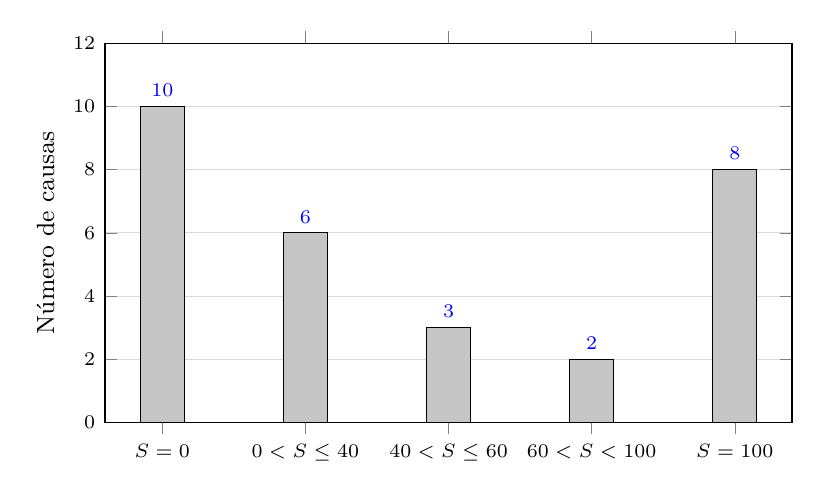
\begin{tikzpicture}
\begin{axis}[
  ybar,
  width=0.85\textwidth, height=6.4cm,
  bar width=16pt,
  ymin=0, ymax=12,
  ylabel={Número de causas},
  ylabel style={font=\small},
  symbolic x coords={{$S=0$},{$0<S\le40$},{$40<S\le60$},{$60<S<100$},{$S=100$}},
  xtick=data,
  x tick label style={font=\scriptsize},
  ytick={0,2,4,6,8,10,12},
  yticklabel style={font=\scriptsize},
  nodes near coords,
  every node near coord/.append style={font=\scriptsize},
  ymajorgrids, major grid style={gray!30},
]
\addplot+[draw=black, fill=gray!45] coordinates
  {({$S=0$},10) ({$0<S\le40$},6) ({$40<S\le60$},3) ({$60<S<100$},2) ({$S=100$},8)};
\end{axis}
\end{tikzpicture}
\caption{Distribución de la salud procesal $S(c)$ en las 29 causas evaluables. La distribución bimodal (10 causas con incumplimiento total de los términos evaluados frente a 8 plenamente puntuales) evidencia gestión procesal heterogénea entre judicaturas.}
\label{fig:hist}
\end{figure}

La Tabla~\ref{tab:causa} ilustra el dictamen completo de una causa representativa, con las cuatro salidas de la arquitectura: veredictos con procedencia normativa, métricas estructurales, cadena de notarización y publicación abierta. Este es el artefacto que las partes procesales y los órganos de control reciben: cada fila es re-derivable por un tercero a partir del expediente público y de $\Omega_L$, cuyo hash acompaña al dictamen.

\begin{table}[H]
\caption{Dictamen integral de la causa 01333202200577 (inquilinato, procedimiento sumario, 10 actuaciones).}
\label{tab:causa}
\begin{tabularx}{\textwidth}{lX}
\toprule
\textbf{Componente} & \textbf{Salida verificable}\\
\midrule
Salud procesal & $S = 65{,}0/100$: 4 términos evaluados, 2 \textsc{cumple}, 1 \textsc{alerta}, 1 \textsc{incumple}.\\
Procedencia & Cada veredicto cita regla, artículo COGEP, fechas comparadas y días hábiles computados (ecuaciones \eqref{eq:habiles}--\eqref{eq:verdict}).\\
Variabilidad fáctica & $\mathrm{IVF} = 57{,}1$: actos fuera del flujo canónico y actos canónicos faltantes (ecuación \eqref{eq:ivf}).\\
Deriva procesal & $\mathrm{IDP} = 25$: un hallazgo de deriva sobre la traza.\\
Notarización & 10 bloques SHA-256 encadenados; raíz publicada; verificación en línea de la cadena (ecuación \eqref{eq:chain}).\\
Datos abiertos & Expediente JSON-LD con 10 acciones tipificadas, DCAT y licencia CC BY 4.0 (Tabla~\ref{tab:opendata}).\\
\bottomrule
\end{tabularx}
\end{table}

\subsection{Análisis de la Garantía de Fidelidad}
La contrapartida de la garantía $\mathcal{H} = 0$ es la cobertura: el sistema responde únicamente dentro del dominio de intenciones tipificadas y de las 11 reglas formalizadas, y rechaza el resto. Frente a las tasas de alucinación del 58--82\% de los LLM generalistas \cite{Dahl2024} y del 17--33\% de las herramientas RAG comerciales \cite{Magesh2025}, este compromiso invierte la carga: la ampliación de cobertura exige formalizar más reglas en $\Omega_L$ ---un proceso auditable de ingeniería del conocimiento \cite{Uschold1996}--- en lugar de tolerar error generativo no acotado. En un dominio donde una cita inexistente puede viciar una actuación procesal, sostenemos con Rudin \cite{Rudin2019} que esta es la dirección correcta del compromiso.

%% ============================================================
\section{Discusión}
\label{sec:discussion}

\textbf{Transparencia jurídica operativa.} La combinación de los tres mecanismos produce una propiedad emergente: la \emph{re-derivabilidad total} del dictamen. Cualquier parte procesal, órgano de control o investigador puede (i) descargar el expediente abierto, (ii) obtener $\Omega_L$ y verificar su hash, (iii) re-ejecutar el razonador determinista y (iv) validar la cadena de notarización. La transparencia no se declara: se puede comprobar computacionalmente, lo que responde a los déficits de confianza documentados en los sistemas de e-justicia \cite{Rosa2013,Lupo2014}.

\textbf{Del hallazgo empírico a la política judicial.} Que solo el 36{,}7\% de los términos evaluados se cumpla, y que el procedimiento sumario rinda peor que el monitorio, convierte al sistema en instrumento de gestión: el ordenamiento de causas por riesgo $\rho(c)$ (ecuación \eqref{eq:riesgo}) prioriza la intervención de los órganos disciplinarios y de apoyo, y la serie temporal de salud por judicatura habilita evaluación comparativa continua, extendiendo al ámbito procesal la lógica de mejora de procesos \cite{Aalst2013}.

\textbf{Limitaciones.} Primero, la garantía de fidelidad es relativa a $\Omega_L$: errores en la formalización de las reglas se propagan a los dictámenes, por lo que la base normativa requiere validación por juristas y control de versiones público (su hash acompaña cada dictamen precisamente para eso). Segundo, la cobertura actual (11 reglas, procedimientos civiles) es una fracción del COGEP; la extensión a otras materias es trabajo de ingeniería del conocimiento, no de arquitectura. Tercero, el libro mayor implementado es una cadena de hashes centralizada con raíz publicable; el anclaje periódico en una DLT permisionada interinstitucional \cite{Olnes2017,Zheng2018} eliminaría la confianza residual en el operador de la plataforma, y la codificación de términos procesales como contratos inteligentes declarativos \cite{Governatori2018,Christidis2016} permitiría alertas automáticas entre instituciones. Cuarto, el corpus (47 causas, dos procedimientos dominantes) es suficiente para demostrar la arquitectura pero no para inferencia estadística sobre la judicatura ecuatoriana; el muestreo estratificado nacional es la extensión natural. Quinto, los índices IVF e IDP detectan desviación estructural pero no distinguen la desviación patológica de la jurídicamente justificada (suspensiones legítimas, acumulaciones); su interpretación exige al operador humano que la arquitectura deliberadamente preserva.

%% ============================================================
\section{Conclusiones y Trabajo Futuro}
\label{sec:conclusions}

Este artículo presentó MALTG-WF, una arquitectura de justicia electrónica que ofrece tres garantías verificables sobre el flujo procesal: fidelidad normativa por construcción (el contenido jurídico emitido pertenece al cierre lógico de una ontología ejecutable del COGEP, con tasa de alucinación nula sobre el dominio tipificado y procedencia criptográficamente trazable), integridad del expediente (cadena de hashes SHA-256 con evidencia de manipulación demostrada) e interoperabilidad semántica (publicación JSON-LD/DCAT conforme a principios FAIR). La evaluación con 47 causas reales instanció el gemelo de flujo del procedimiento sumario (171 actividades, 79 flujos), evaluó 60 términos procesales y produjo un diagnóstico accionable: puntualidad del 36{,}7\%, salud procesal media de 44{,}4/100 y desviación estructural generalizada respecto al flujo canónico.

El trabajo futuro comprende: (i) la ampliación de $\Omega_L$ a más materias y recursos del COGEP con validación por panel de juristas; (ii) el anclaje de las raíces de notarización en una red DLT permisionada compartida por el ecosistema de justicia (judicatura, defensoría, fiscalía) \cite{Olnes2017}; (iii) la incorporación controlada de LLM para la interpretación de consultas $\iota$ y el resumen de documentos, manteniendo la barrera sobre el contenido jurídico y midiendo $\mathcal{H}$ con protocolos de evaluación estandarizados \cite{Huang2025}; y (iv) el escalamiento del corpus para estudios longitudinales de política judicial con la infraestructura de datos abiertos aquí propuesta.

\vspace{6pt}

\authorcontributions{Conceptualización, metodología, software, validación, redacción: P.M.A. El autor ha leído y aceptado la versión publicada del manuscrito.}

\funding{Esta investigación no recibió financiación externa.}

\institutionalreview{No aplicable. Los expedientes procesados son registros públicos accesibles a través del sistema oficial de consulta de procesos judiciales del Ecuador.}

\informedconsent{No aplicable.}

\dataavailability{El código fuente de la plataforma MALTG, la base de conocimiento COGEP (con su hash de versión), el gemelo de flujo BPMN y los expedientes JSON-LD están disponibles a solicitud al autor de correspondencia. Los datos procesales proceden del sistema público de consulta de procesos judiciales del Consejo de la Judicatura del Ecuador.}

\conflictsofinterest{El autor declara no tener conflictos de interés. Los indicadores generados por el sistema son instrumentos de apoyo a la gestión y no constituyen asesoría jurídica ni prejuzgan la conducta procesal de los intervinientes.}

%% ============================================================
\begin{adjustwidth}{-\extralength}{0cm}
\reftitle{Referencias}
\bibliography{references}
\end{adjustwidth}

\end{document}
